\section{Methodology: Decoupled Namespaces}
\label{sec:methodology-decoupled-namespaces}

\begin{figure}[tb]
\caption{Applications can decouple the namespace, write updates to a local
journal, and delay metadata updates.  Table~\ref{table:spectrum} shows how
these phases (represented by the arrows) can be combined to provide weaker
consistency or fault tolerance semantics.  }\label{fig:decouple}
\centering
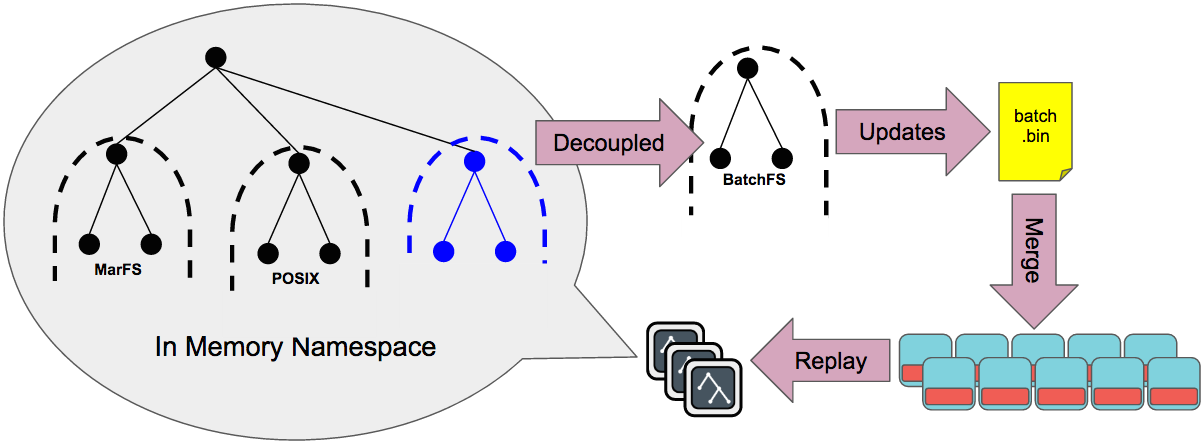
\includegraphics[width=90mm]{figures/fig-decouple.png}
\end{figure}

In this section we describe Cudele, our prototype system that lets future
programmers compose mechanisms (Section~\S\ref{sec:cudeles-mechanisms}) to
provide the necessary guarantees
(Section~\S\ref{sec:setting-policies-with-cudele}) for their application.

\subsection{Cudele's Mechanisms}
\label{sec:cudeles-mechanisms}

% describe the figure
Figure~\ref{fig:decouple} shows the mechanisms (labeled arrows) in Cudele and
which entity they are performed by (gray boxes). The metadata store and journal
are different ways of representing the namespace. The metadata store represents
the namespace as a tree of directory fragments and is easier to read/traverse.
On the other hand, the journal represent the namespace as a list of events. It
a ``pile system"; writes are fast but reads are slow because state must be
reconstructed.  Specifically, reads are slow because there is more data to
read, it is unorganized, and many of the updates may be redundant.

% describe the mechanisms
Cudele presents 6 mechanisms: RPCs, Stream, Create, Volatile Apply, Save, and
Persist. ``RPCs" does round trip remote procedure calls to establish
consistency; it is the default implementation for complying with POSIX in
CephFS. ``Stream" has the metadata servers stream a journal of metadata updates
into the object store. ``Create" allows clients to append metadata events to an
in-memory journal. ``Volatile apply" takes the in-memory journal on the client
and applies it directly to the in-memory metadata store of the metadata server
cluster. ``Save" takes the in-memory journal and writes it to the client's
disk. ``Persist" saves the journal as a an object in the object store from the
client.

Next, we discuss how these mechanisms can be composed to get different
consistency and fault tolerance semantics. 

%\begin{tabular}{ r | l }
%  \(\Rightarrow\)   & Description \\\hline
%  create            & events appended to in-memory journal \\
%  v\_apply           & journal volatily applied to in-memory metadata store \\
%  save              & journal saved to client's disk \\
%  persist           & journal saved in object store \\
%  replay            & metadata servers materialize namespace \\
%  RPCs              & round trip remote procedure calls \\
%  stream            & metadata server streams journal into RADOS \\
%\end{tabular}

\subsection{Setting Policies with Cudele}
\label{sec:setting-policies-with-cudele}

\begin{table}[t]
\begin{center}
\caption{Future programmers can explore the consistency (C) and
durability (D) spectrums by composing Cudele mechanisms. The consistency
and durability properties are not guaranteed until all mechanisms in the cell
are complete (i.e. the compositions should be considered atomic) and there are
no guarantees while tranisitioning between policies. \label{table:spectrum}}
\begin{tabular}{ l | l | l | l }
  Consistency \(\rightarrow\) &&& \\  
  Durability \(\downarrow\)  & invisible         & eventual        & strong  \\\hline
  none                       & create            & create          & RPCs    \\
                             &                   & +volatile apply &         \\\hdashline
  local                      & create            & create          & RPCs    \\
                             & +local persist    & +local persist  & +local  \\
                             &                   & +volatile apply &  persist\\\hdashline
  global                     & create            & create          & RPCs    \\
                             & +global persist   & +global persist & +stream \\
                             &                   & +volatile apply &         \\
\end{tabular}
\end{center}
\end{table}

% describe table
The spectrum of consistency and fault tolerance guarantees that adminstrators
can construct is shown in Table~\ref{table:spectrum}. The columns are the
different consistency semantics and the rows cover the spectrum of fault
tolerance guantees. For consistency: ``none" means the system does not handle
merging updates into a global namespace and it is assumed that middleware or
the application manages consistency lazily; ``eventual" merges updates either
when the system has time (e.g., by a background daemon) or when the client is
done writing; and updates in ``global" consistency are seen immediately by all
clients. For fault tolerance, ``none" means that updates are volatile and will
be lost on a crash of any component. Stronger guarantees are made with
``local", which means updates will be retained if the client node recovers, and
``global", where all updates are always recoverable.

% which system they represent and which are impossible
The cells in Table~\ref{table:spectrum} encompass many exisiting storage
systems. POSIX systems like CephFS and IndexFS have global consistency and
fault tolerance; DeltaFS has consistency and fault tolerance set to ``none";
and BatchFS uses ``eventual" consistency and ``local" fault tolerance. These
are just a few of the HPC examples.  

% how its done
To compose the mechanisms administrators inject which steps (described in
Section~\S\ref{sec:cudeles-mechanisms}) to run and which to use in parallel
using a domain specific language. For example, to get the semantics of BatchFS,
the administrator would inject the following pipeline:\\

\noindent \texttt{create+save+volatile apply}\\

% what is impossible
Although we can achieve all permutations of the different guarantees in
Table~\ref{table:spectrum}, not all of them make much sense. For example, it
makes little sense to do \texttt{creates+RPCs} since both steps do the same
thing or \texttt{stream+save} since global fault tolerance is stronger and has
more overhead than local fault tolerance.  Formulaically, valid steps
include:\\

\noindent \texttt{<create|RPCs> [+v\_apply][+save][+persist][+stream]}

\subsection{Cudele Namespace API:\\Per-Subtree Policies}

% file type
To assign consistency and fault tolerance to the subtrees we store policies in
the directory inode. This approach uses the File Type interface from the
Malacology programmable store system~\cite{} and it tells clients how to access
the underlying data or metadata. The underlying implementation stores
executable code in the inode that calls the different Cudele mechanisms. Of
course, there are many security and access control aspects of this approach but
that is beyond the scope of this paper.

% the interface
The interface for setting the subtree policies is with \{path,
<block|overwrite>, pre-allocated inodes\} tuples. For example:

\texttt{(msevilla/mydir, policies.yml)}

would decouple the path \texttt{msevilla/mydir} and would apply the policies in
\texttt{policies.txt}. The policies file supports the following values:

\begin{itemize}

  \item \texttt{allocated\_inodes}: the number of inodes to allocate to the
  decoupled namespace (default 100)

  \item \texttt{interfere\_callback}: how to handle a request from another
  client targeted at the now decoupled subtree (default \texttt{block})

  \item \texttt{consistency\_callback}: which consistency model to use (default
  \texttt{RPCs})

  \item \texttt{durability\_callback}: which durability model to use (default
  \texttt{stream})

\end{itemize}

Given these default values decoupling the namespace with an empty policies file
would give the application 100 inodes but the subtree would behave like the
existing CephFS implementation. Table~\ref{} shows how one would use the Cudele
API to implement policies from related work. 


%

For \texttt{block}, any requests to this part of the namespace return with
``Device is busy", which will spare the MDS from wasting resources for updates
that may get overwritten. If the application does not mind losing updates, for
example it wants approximations for results that take too long to compute, it
can select \texttt{overwrite}. In this case, metadata will be written and the
computation from the decoupled namespace will take priority because the resutls
are more accurate.

\begin{listing}
\begin{minted}[frame=single,
               framesep=3mm,
               xleftmargin=21pt,
               tabsize=4]{js}
{     
    "allocated_inodes": "100000"
    "interfere_policy": "block"
    "consistency": "create"
    "durability": "local_persist"
}
\end{minted}
\caption{Implementing DeltaFS with Cudele.}
\label{src:deltafs}
\end{listing}

\begin{listing}
\begin{minted}[frame=single,
               framesep=3mm,
               xleftmargin=21pt,
               tabsize=4]{js}
{     
    "allocated_inodes": "100000"
    "interfere_policy": "block"
    "consistency": "create+volatile_apply"
    "durability": "local_persist"
}
\end{minted}
\caption{Implementing BatchFS with Cudele.}
\label{src:batchfs}
\end{listing}

\begin{listing}
\begin{minted}[frame=single,
               framesep=3mm,
               xleftmargin=21pt,
               tabsize=4]{js}
{     
    "allocated_inodes": "-"
    "interfere_policy": "-"
    "consistency": "RPCs"
    "durability": "stream"
}
\end{minted}
\caption{Existing CephFS on Cudele.}
\label{src:batchfs}
\end{listing}

% // limit consistency
% if metadata write (create) -- try to reduce error bars for many creates and runtime of one touch)
%   if !RPCs
%     if overwrite
%       do nothing and let the RPC go
%     else
%       return -EBUSY
%
% // limit fault tolerance
% if !stream
%   return immediately on mdlog


